% 26/09 - 29/09
%------------------
% INTRODUCTION 
%------------------

\section{Introduction}
The course will deal with two types of situations :
\begin{enumerate}
\item Analysis and modelling of \textbf{Time-Series}
\item Analysis and modelling of \textbf{Input/Output Systems}
\end{enumerate}
%-----------------------------------------------------------------------------------%
%-----------------------------------------------------------------------------------%

\subsection{Time-Series} 
Time series consider vectors  $\{y(1), y(2) , ... , y(N)\}$  of \textbf{measured data} of cardinality N ( large , 1000 - 10000).\\
Said vectors are considered in the \textbf{time-domain} : y(t) is a signal or \textbf{stochastic process} generated by the system whose output is than sampled.

\begin{figure}[!h]
\begin{minipage}{.5\textwidth}
  \centering
  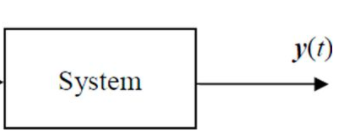
\includegraphics[width=.7\linewidth]{ts_system}
\end{minipage}%
  \begin{minipage}{.5\textwidth}
  \centering
  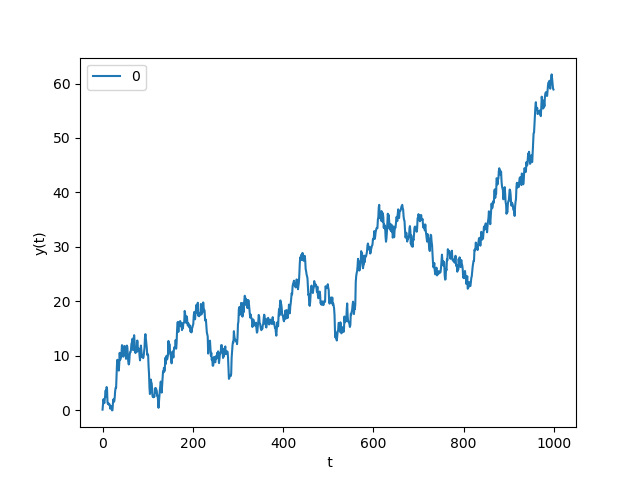
\includegraphics[width=.7\linewidth]{ts}
\end{minipage}%
\end{figure}
%-----------------------------------------------------------------------------------%

\subsubsection{TS Applications}
TS are used for two problems : 
\begin{enumerate}
\item \textbf{Prediction problem} : $\{ y(1) ... y(N) \} \rightarrow \hat{y} (\frac{N+K}{N})$ \\ Given N measurements \textbf{estimate} the measurement K timesteps ahead
\item \textbf{Filtering problem} : $\{ x_1(t) ... x_N(t) \} \rightarrow \hat{x} (\frac{t}{t})$ \\Where $\{ x_1(t) ... x_N(t) \}$ are internal variables of the system
\end{enumerate}
\vfill
%-----------------------------------------------------------------------------------%
%-----------------------------------------------------------------------------------%

\subsection{I/O Systems} % Sub-section
I/O systems consider two measurements : 
\begin{itemize}
\item \textbf{Input} : $\{ u(1) ... u(N) \} $
\item \textbf{Output}: $\{ y(1) ... y(N) \} $
\end{itemize}
Resulting in two signals u(t) and y(t). 
Input signal $ u(t) $ can be of two types: 
\begin{easylist}[itemize]
\ListProperties(Hide=100, Hang=true, Progressive=3ex, Style*=--)
& \textbf{Controllable} : can be affected ( ex : voltage )
& \textbf{Uncontrollable} : cannot be affected ( ex : rain )
\end{easylist}

\begin{figure}[!h]
  \centering
  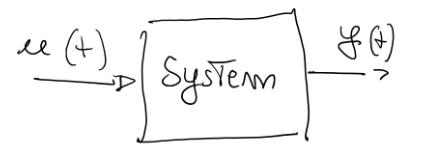
\includegraphics[width=.5\linewidth]{IO}
\end{figure}
%-----------------------------------------------------------------------------------%

\subsubsection{I/O Applications}
I/O systems are used for three problems : 
\begin{enumerate}
\item \textbf{Prediction problem} : $\{ y(1) ... y(N) \} \rightarrow \hat{y} (\frac{N+K}{N})$ \\ Given N measurements \textbf{estimate} the measurement K timesteps ahead
\item \textbf{Filtering problem} : $\{ x_1(t) ... x_N(t) \} \rightarrow \hat{x} (\frac{t}{t})$ \\Where $\{ x_1(t) ... x_N(t) \}$ are internal variables of the system
\item \textbf{System control problem} : given a desired output $ \bar{y}(t) $ , control $ u(t) $ so that $y(t)$ is as close as possible to  $ \bar{y}(t) $
\end{enumerate}

\begin{figure}[!h]
  \centering
  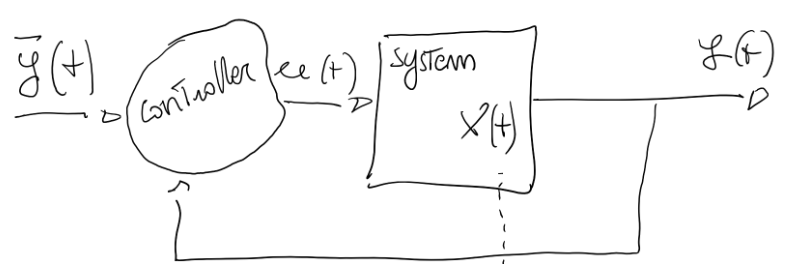
\includegraphics[width=.6\linewidth]{IO_control}
\end{figure}
%-----------------------------------------------------------------------------------%
%-----------------------------------------------------------------------------------%

\subsection{Time Series vs I/O Systems} % Sub-sub-section
In prediction and filtering problems both I/O systems and TS can be used. 
How to chose which one to use?
\begin{description} % Numbered list example

\item[Ex.1] \hfill \\
- \textbf{System} : Electric Motor \\
- \textbf{Input} :  Current , temperature of motor,electromagnetic fields nearby..  \\
- \textbf{Output} : Torque \\
We can say that our main input variable (current) is responsible for 90\% of the output.The other variables only have slight effects on the torque so they are considered \textbf{noise} \\
The best model to choose is the \textbf{I/O}
\item[Ex.1] \hfill \\
- \textbf{System} : Macro-Economic System \\
- \textbf{Input} :  Too many  \\
- \textbf{Output} : Stock prices of FCA \\
There are many thousand variables affecting the output. Listing and measuring them all would make the model too complex . In this case all the input variables are considered \textbf{noise} : the best model to choose is the \textbf{Time Series}
\item[Ex.3] \hfill \\
- \textbf{System} : Environment \\
- \textbf{Input} :  Rain, wind, heatings, cars , temperature, pressure... \\
- \textbf{Output} : PM10 levels \\
In this case some main inputs variables can be selected ( ex :cars , heating and rain ) while the others are modelled as noise. In this case \textbf{I/O} model should be used. \\ It is not wrong to consider all the inputs as noise and model the problem as \textbf{Time Series}.
\end{description} 
\newpage
General rule:
\begin{table}[!ht]
\centering
\label{my-label}
\begin{tabular}{lllll}
\cline{1-2}
\multicolumn{1}{|l|}{}    & \multicolumn{1}{l|}{Advantages}                 &  &  &  \\ \cline{1-2}
\multicolumn{1}{|l|}{TS}  & \multicolumn{1}{l|}{Only y(t) must be measured} &  &  &  \\ \cline{1-2}
\multicolumn{1}{|l|}{I/O} & \multicolumn{1}{l|}{Better estimation}          &  &  &  \\ \cline{1-2}
                          &                                                 &  &  & 
\end{tabular}
\end{table}


%-----------------------------------------------------------------------------------%
%-----------------------------------------------------------------------------------%

\subsection{Modelling structures}
Depending on the problem 2 modelling structures are used.\\
The TS are modelled with a \textbf{mathematical model} which outputs signal
$y(t)$. An \textbf{imaginary} input $ e(t) $ called \textbf{white noise} is considered as \textbf{standard input} and it is \textbf{part of the model}.\\
The I/O system is modelled by two \textbf{mathematical models} which output signal $ y(t) $.  As above \textbf{white noise} is considered as input of one of the two models. The other model has input $ u(t) $ which is \textbf{not} part of the model.\\

\begin{figure}[!h]
\begin{minipage}{.5\textwidth}
  \centering
  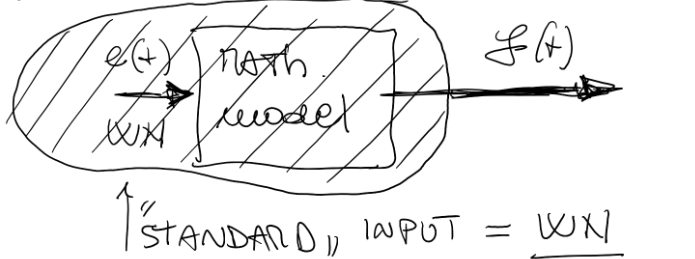
\includegraphics[width=.7\linewidth]{ts_model}
  \caption{TS Model}
\end{minipage}%
  \begin{minipage}{.5\textwidth}
  \centering
  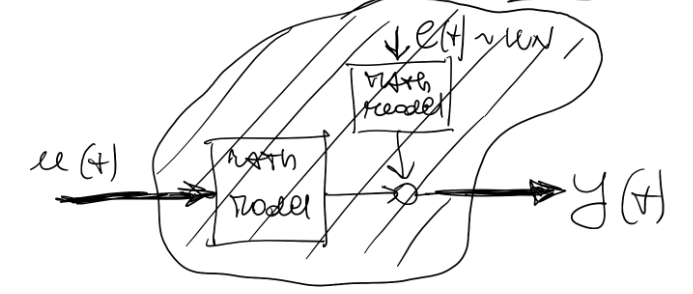
\includegraphics[width=.7\linewidth]{io_model}
  \caption{IO Model}
\end{minipage}%
\end{figure}

All signals and systems are \textbf{time-discrete} . Analogue signals are converted to digital signals through \textbf{ADCs} . \\Discrete time points are spaced evenly at pace $ \Delta T $ = sampling time

\newpage
\subsection{Mathematical Models}
The mathematical models used to elaborate output functions are either \textbf{white boxes} or \textbf{black - boxes}.
\begin{figure}[!h]
  \centering
  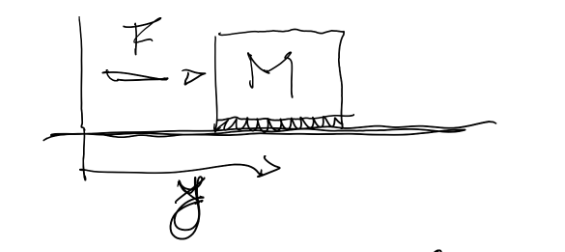
\includegraphics[width=.5\linewidth]{massmodel}
  \caption{System to be modelled}
\end{figure}
%-----------------------------------------------------------------------------------%

\subsubsection{White Box Models}
Also called \textit{first-principles models} assume that the parameters involved in the system are known and well defined. Using white box models we get a \textbf{physical interpretation of the model} which makes them useful if the aim is to design the system.\\
In the example we can derive laws that define our system's \textbf{transfer function} given as input a force $ \vec{F} $ and output $ y $ :  $$ \ddot yM = F - c \dot y \rightarrow Laplace \rightarrow  s^2My = F -scy $$ $$ (s^2M + sc )y = F $$ $$ y = \frac{1}{s^2M + sc} F $$
%-----------------------------------------------------------------------------------%

\subsubsection{Black Box Models}
In black box models we don't know the internal parameters that influence the system. 
In our example , we only know that by changing the input $ \vec{F} $ a corresponding change in output $ y(t) $ can be measured . By measuring the data we can derive a model :  $$ y(t) =  \frac{b_0Z^2 + b_1Z+ b_2}{a_0Z^2 + a_1Z + a_2} F(t) $$ where 
$ a_0,...,a_2 , b_0 ,..., b_2  $ are the parameters. 
%-----------------------------------------------------------------------------------%

\subsubsection{White box vs Black box}
\begin{table}[!h]
\centering
\caption{WB/BB Comparison}
\label{my-label}
\begin{tabular}{lllll}
\cline{1-2}
\multicolumn{1}{|c|}{White Box}                                                                                                                                    & \multicolumn{1}{c|}{Black Box}                                                                                                                                &  &  &  \\ \cline{1-2}
\multicolumn{1}{|l|}{\begin{tabular}[c]{@{}l@{}}-Get physical interpretation of the model\\  and its parameters. \\ -Useful for designing the system\end{tabular}} & \multicolumn{1}{l|}{\begin{tabular}[c]{@{}l@{}}-Very fast\\ -Very accurate\\ -Does not require know-how of the domain\\ -Can be easily re-tuned\end{tabular}} &  &  &  \\ \cline{1-2}
                                                                                                                                                                   &                                                                                                                                                               &  &  & 
\end{tabular}
\end{table}
%-----------------------------------------------------------------------------------%
%----------------------------------------------------------------------------------------
\subsection{Stochastic Processes}
\begin{description}
\item[Random variable RV:] \hfill \\ $ v(s) $ is completely defined by its probability distribution ( Gaussian, Uniform...) which is related to its \textbf{probability density function } ( PDF )
\item[Stochastic Process:] \hfill \\ is a sequence of \textbf{time-ordered random variables} defined at the same experiment S  $$ v(1,S) , v(2,S) ,..., v(t,S)  $$ where t is the time index. If the experiment is \textbf{fixed} $ S = \bar{S} $ , we get an instance , a \textbf{realisation} of the stochastic process : $$ v(1,\bar{S}), ... ,v(t,\bar{S}) $$ resulting in a set of samples  $ \{y(1),...,y(N) \} =  \{y(1, \bar{S}),...,y(N ,\bar{S}) \} $
\end{description}
%-----------------------------------------------------------------------------------%

\subsubsection{Characteristics}
\begin{description}
\item[Mean value m(t):] \hfill\\
expected value of a random variable v(t,S) at time t  $$ m(t) = E [v(t,S)]$$
\item[Covariance Function $ \gamma(t_1,t_2)$:] \hfill \\
expected value of the \textbf{product} of two \textbf{unbiased} random variables at time instants t1, t2 :$$ \gamma(t_1,t_2) : E[ ( v(t_1,S) - m(t_1))(v(t_2,S)-m(t_2))] $$
Removing the mean brings the signal closer to 0.\\ If t1 = t2 = t the covariance degenerates in \textbf{variance}: $$ \gamma(t) = E [ (v(t,S)- m(t))^2] $$ 
\end{description}
 %-----------------------------------------------------------------------------------%

\subsubsection{Stationary Stochastic Processes}
Has properties:
\begin{enumerate}
\item $ m(t) = m , \forall t$
\item $ \gamma(t_1,t_2) $ depends on $ \tau = | t_1 - t_2 | $ \\ This means that the covariance depends on the \textbf{distance in time} and not on specific considered samples.\\ 
   $ \gamma(t_1,t_2)= \gamma(t_3,t_4) \rightarrow |t_1-t_2|=|t_3-t_4|$ \\
   $ \gamma(\tau) = E[ (v(t) - m)(v(t-\tau)-m)] $ has properties :
   \begin{itemize}
   \item $ \gamma(0) = E[(v(t)-m)^2] \rightarrow$ \textbf{variance}
   \item $ |\gamma(\tau)| \leq \gamma(0) $
   \item $ \gamma(\tau) = \gamma(- \tau)$
   \end{itemize}
\end{enumerate}
\begin{description}
\item[SSP Equivalence]\hfill\\
Two SSPs $y_1(t) , y_2(t)$ are equivalent in a \textbf{weak sense} if:
\begin{itemize}
\item $m_{y1} = m_{y2}$
\item $\gamma_{y1}(\tau) = \gamma_{y2}(\tau)  $ ,$\forall \tau$
\end{itemize}
\newpage
\item[Correlation Function]\hfill\\
If the $ m = 0 $ the $ \gamma(\tau) $ function degenerates in the \textbf{correlation function} : $$ E[v(t)v(t-\tau)] $$
\begin{figure}[!h]
  \centering
  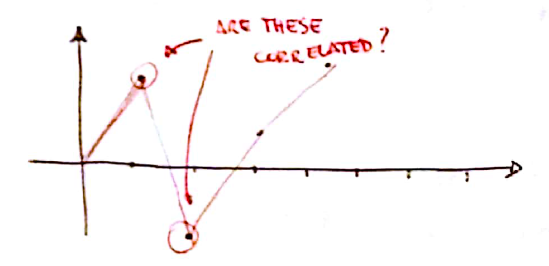
\includegraphics[width=.5\linewidth]{correlation}
\end{figure}
\end{description}
%-----------------------------------------------------------------------------------%

\subsubsection{White Noise}
e(t) is SSP called \textbf{white noise} and is written as $$ e(t) \rightarrow WN(\mu , \lambda^2) $$
Properties: 
\begin{itemize}
\item Mean value : $ E[e(t)] = \mu , \forall t $
\item Variance : $ \gamma_e(0) = E[ (e(t)- \mu)^2] = \lambda^2 $
\item Covariance : $ E[(e(t)-\mu)(e(t-\tau)-\mu)] = 0 $ , $ \forall t, \forall \tau \neq 0 $f
\begin{figure}[!h]
  \centering
  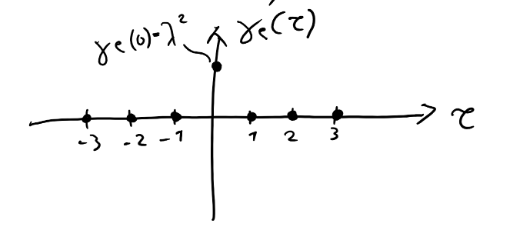
\includegraphics[width=.7\linewidth]{no_cov}
\end{figure}
\end{itemize}
No covariance means that the samples are \textbf{not related}\\
Considering a \textbf{Gaussian Distribution}  : $ e(t) \rightarrow WGN ( \mu, \lambda^2) $

\newpage
%-----------------------------------------------------------------------------------%
%-----------------------------------------------------------------------------------%

\subsection{Sample estimation of mean and covariance function}
Dealing with samples it is useful to \textbf{estimate} the mean and covariance of the samples.\\ Output y(t) is a SSP : $ \{ y(1) ,...,y(N)\}$ a particular realisation of $ \bar{S}$ with :\\ 
\begin{itemize}
\item Mean $ m = E[y(t)]$
\item Covariance $ \gamma(\tau)= E[(y(t)-m)(y(t-\tau)-m)] $ 
\end{itemize}
This seems trivial but the computation of the expected value cannot be done because the \textbf{distribution of the process} is \textbf{unkown}.\\
These two can be \textbf{estimated}



%-----------------------------------------------------------------------------------%
\subsubsection{Sample Mean}
The sample mean is a good estimator for the mean m : $$ \hat{m}_n = \frac{1}{N} \sum\limits_{t=1}^N y(t) $$
Properties of the estimator : 
\begin{enumerate}
%-----CORRECTNESS -------%
\item $ \hat{m}_n $ is \textbf{correct} if $ E[\hat{m}_n] = m $\\
\textbf{Proof}: $ E[\hat{m}_n] = E[\frac{1}{N} \sum\limits_{t=1}^N y(t,s)] = 
\frac{1}{N} \sum\limits_{t=1}^NE[y(t,s)] = \frac{1}{N} \sum\limits_{t=1}^N m =$\textbf{m} 
\begin{description}
\item[Example]\hfill \\
$y(t,S) = \bar{v}(s) \rightarrow WN(0,1) $ and $ S = \bar{S} , \{ y(1,\bar{S}),...,y(N,\bar{S} \}$ so :\\ 
-$ \hat{m}_n = \frac{1}{N} \sum\limits_{t=1}^N y(t,\bar{S}) = \frac{1}{N} \sum\limits_{t=1}^N \bar{v}(\bar{S}) = \frac{1}{N} N \bar{v}(\bar{S}) \neq 0 \rightarrow$ bad estimator\\
-$ \breve{m}_n = \frac{1}{N} \sum\limits_{S=1}^N y(\bar{t},S) = \frac{1}{N} v(S) \to  0 \rightarrow$ good estimator \\
\end{description}
%-----COSISTENTCY ----%
\item $ \hat{m}_n $ is \textbf{consistent} if $ E[(\hat{m}_n - m )^2] \xrightarrow[N \to \infty] {} 0 $ \\ The \textbf{error variance} approaches 0 for large values of N: this means that with a lot of data $N \to \infty$ we can estimate $\hat{m}_n$ more effectively. 
\\In general one can say that  $\hat{m}_n$ is consistent if  $\gamma(\tau) \xrightarrow[|\tau| \to \infty] {} 0$
\begin{description}
\item[Example]\hfill \\
$ y(t,S) = \bar{V}(S) \to WN(0,1) $ \\ $ \gamma(\tau)=  E[(\gamma(\tau))(\gamma(t-\tau))] = E[ \bar{V}(S) \bar{V}(S)] = E[\bar{V}(S)^2] = 1 $ 
\end{description}
\end{enumerate}

%-----------------------------------------------------------------------------------%
\subsubsection{Sample Covariance}
y(t) is a SSP with \textbf{zero mean}.\\
A good estimator for for the covariance is the \textbf{sample covariance}:
$$ \hat{\gamma}_N(\tau)	= \frac{1}{N-\tau} \sum\limits_{t=1}^{N-\tau}y(t)y(t+\tau)$$ $$ 0 \leq \tau \leq N-1$$
It is important to notice that this approximation is good for $ \tau << N $ because the accuracy of $ \gamma_N(\tau) $ \textbf{decreases} with $ \tau $ \\
Properties of the estimator :
\begin{enumerate}
\item $ \hat{\gamma}_N(\tau)$ is \textbf{correct} if $ E[ \hat{\gamma}_N(\tau)] = \mathbf{\gamma(\tau) }$ 
\begin{description}
\item[Proof:]\hfill\\
$ E[ \hat{\gamma}_N(\tau)] = E[ \frac{1}{N-\tau} \sum\limits_{t=1}^{N-\tau}y(t)y(t+\tau)]  = \frac{1}{N-\tau} \sum\limits_{t=1}^{N-\tau} E[y(t)y(t+\tau)] = \frac{1}{N-\tau} \sum\limits_{t=1}^{N-\tau} \gamma(\tau) = \gamma(\tau) $
\end{description}
\item $\hat{\gamma}_N(\tau)$ is \textbf{consistent} if $ E[(\hat{\gamma}_N(\tau)-\gamma(\tau))^2] \xrightarrow[N \to \infty] {} 0 $ , \\ \textbf{True } if $ \gamma(\tau) \xrightarrow[|\tau| \to \infty]{} 0$
\end{enumerate}
\begin{description}
\item[Observation 1:]\hfill\\
$ \hat{\gamma}_N(\tau)	= \frac{1}{N-\tau} \sum\limits_{t=1}^{N-\tau}y(t)y(t+\tau) $ \\ $ 0 \leq \tau \leq N-1 , \tau \geq 0$ \\ but since y(t) is a SSP $ \gamma(\tau) = \gamma(-\tau) $ : $$ \hat{\gamma}_N(\tau)	= \frac{1}{N-|\tau|} \sum\limits_{t=1}^{N-|\tau|}y(t)y(t+|\tau|) $$ $$ |\tau| \leq N-1 $$ 
\newpage
\item[Observation 2:]\hfill\\
$ \hat{\gamma}_{N}'(\tau)	= \frac{1}{N-|\tau|} \sum\limits_{t=1}^{N-|\tau|}y(t)y(t+|\tau|) \to E[ \hat{\gamma}_{N}'(\tau)] = ... = \frac{1}{N} \gamma(\tau)(N-|\tau|) $\\As shown $ \hat{\gamma}_{N}'(\tau)$  \textbf{doest not} satisfy the \textbf{correct} property.\\However for N $\to \infty $ and $ \tau << N $ :  $ \hat{\gamma}_{N}'(\tau)$ is \textbf{asimptotically correct}
\end{description}